%----------------------------------------------------------------------------------------
%	SECTION 5
%----------------------------------------------------------------------------------------
\newpage
\section{Engineering Practice (P)}


\subsection*{P1(i, -)}

\begin{wraptable}[10]{r}{0.2\textwidth}
    \begin{tabular}{|ll|}
        \hline
        \multicolumn{2}{|c|}{\cellcolor[HTML]{F8A102}\textbf{P1(i, -)} \nomaster} \\ \hline
        \BST & \IE \\
        \DPA & \Acoustics \\
        \EnvBeh & \EPA \\
        \DPB & \CAS \\
        \ELS & \EnBldgs \\
        \TPS & \DI \\
        \FMP & \PRJ \\
        \DST & \LAB \\
        \SIB & \CCSA \\
        \WSD &  \\
        Arup & Hoare Lea \\
        Sunamp & Sweco \\ \hline
    \end{tabular}
\end{wraptable}

Throughout the programme, I have gained knowledge and understanding of some contexts in which my AE knowledge can be applied.
The following list, in which I describe such contexts, is not exhaustive.

\begin{enumerate}
	\item %The collaborative design projects in years \hl{1/2} and 4,
	%\textit{Building Services Technology},
	%\textit{Introduction to the Environment},
	%\textit{Design Project A},
	%\textit{Design Project B},
	%\textit{Electrical and Lighting Services for Buildings},
	%\textit{Critical Architectural Studies},
	%\textit{Design Project},  
	Several courses throughout the years and my placements at Arup and Hoare Lea
	provided me with the practical experience of applying my AE knowledge in the context of a team designing a building and/ or its services, in which I was responsible for the building services, the building's internal environment and the occupants' comfort levels.
	My group's first prize for sustainability (see Figure~\ref{fig_award}) demonstrates my understanding of an Architectural Engineer's role in passive design (e.g. natural lighting).
	
	\item Throughout several courses (especially \FMPTitle),
	%\textit{Acoustics and Architectural Design},
	%\textit{Environment and Behaviour},
	%\textit{Energy Principles and Applications},
	%\textit{Energy and Buildings},
	%\textit{Thermal Performance Studies},
	%\textit{Design Issues},
	%\textit{Facilities Management Principles},
	%\textit{Laboratory Project},
	%\textit{Sustainable and Intelligent Buildings},
	%\textit{Climate Change, Sustainability and Adaptation},
	%\textit{Water Supply and Drainage for Buildings},
	my work in the environmental certification of existing buildings at Sweco,
	and
	my encounter with a specialist in Performance at Hoare Lea,
	%Design Issues,
	I have also learned that my AE knowledge is applicable in the operation and management of buildings and building services (a.k.a. facilities management) to, for example, improve the occupants' comfort levels, optimise performance or increase resilience to future impacts of climate change.
	
	\item Through the work I did at Sunamp as well as my encounter with a technical author at Hoare Lea, I understand that engineering knowledge is important in the composition of technical documents (e.g. specifications, operation and maintenance manuals) and even marketing material for technical products, which may need to explain engineering processes graphically and in layman's terms.
	See how I did this in the UniQ PISs in Appendix~\ref{App:PISs}.
	
	\item My dissertation in particular taught me that engineering knowledge is necessary for the development of industry standards and codes of practice, such as the series of Publicly Available Specifications (PAS) 1192 which standardise the requirements for achieving BIM Level 2.
	
	\item Throughout my dissertation and \textit{Climate Change, Sustainability and Adaptation} (\CCSA), I have also come to understand that my engineering knowledge can be used for research, the development of new technologies or processes, and to influence policies.
	One of the assignments for \CCSA \space was to write a briefing for politicians;
	mine urged them to develop policies to make the existing UK housing stock resilient to future climate impacts.
	%\hl{Repeated DST and CCSA. Could even include Sunamp. Maybe this example is one too many...}
\end{enumerate}




\subsection*{P2(i, b, m)}

\begin{wraptable}[12]{r}{0.2\textwidth}
    \begin{tabular}{|ll|}
        \hline
        \multicolumn{2}{|c|}{\cellcolor[HTML]{F8A102}\textbf{P2(i, b, m)} \nomaster} \\ \hline
        \ConTechOne & \BST \\
        \DPA & \ConTechTwo \\
        \Acoustics & \EnvBeh \\
        \Stats & \DPB \\
        \CAS & \ELS \\
        \DSA & \EnBldgs \\
        \TPS & \PRJ \\
        \DST & \LAB \\
        \SIB & \ICP \\
        H\&L & Arup \\
        Hoare Lea & Sunamp \\ \hline
    \end{tabular}
\end{wraptable}

I have gained knowledge of the characteristics of, an understanding of and an ability to use a range of computer-based tools, engineering processes, and building services products:
\begin{itemize}
    %\item P2i 
     
    % In \textit{Environment and Behaviour}, \textit{Laboratory Project} and \textit{Dissertation}, I developed an ability to use the statistics software tool SPSS (Statistical Package for the Social Science).
    % The course \textit{Statistics for Science} provided me with a foundation to understand the data in the inputs and outputs of this software.
    
    \item \textbf{P2i and P2b}
    
    In \textit{Design Software Applications} and \textit{Laboratory Project}, I gained knowledge of the characteristics of steady-state and dynamic building modelling and energy analysis software programmes, notably iSBEM, SAP, IES, and CFD [\textbf{P2b}].
    As these courses only provided an introduction to these software programmes, I have not mastered my ability to use them [\textbf{P2i}].
    %\hl{Look up} \DSATitle \space \hl{notes if you want to demonstrate knowledge.}
    This was demonstrated during my attempt to model my \textit{Design Project} building in IES; my building model overheated due to variation and temperature profiles that I had incorrectly set up, amongst other things.
    
    %During the \textit{Design Project} and my placements at Hultin \& Lundquist Arkitekter and Sunamp, I gained an understanding of and an ability to use Autocad.
    %Likewise, I learned to use Revit during the \textit{Design Project} and my placements at Arup and Hoare Lea.
    %Although my ability to use these Autodesk products (i.e. Autocad and Revit) is limited, I have learned quite a bit about their characteristics.
    %In \textit{Dissertation} and \textit{Innovation in Construction Practice}, I learned about the prominent use of these products in the UK construction industry and how their proprietary characteristics can lead to problems of interoperability.
    
    Regarding engineering processes, 
    %I have learned extensively about the BIM process in Dissertation and Innovation in Construction Practice.
    I have learned the characteristics of and practised the optimisation process of an engineering design in \textit{Laboratory Project} (see \textit{EA3(i, b, m)} in Section \ref{EA3} for more detail) [\textbf{P2i and P2b}].
    
    \item \textbf{P2m}
    
    Throughout many of my construction-based courses and my placements at Sunamp, Hoare Lea and Arup,
    I have accumulated an extensive knowledge of a wide range of building services products (e.g. heat pumps, heat batteries, PV panels) and building materials (e.g. PCMs, Ziegel blocks, steel).
    My understanding of these products and materials, however, varies.
    %\hl{Elaborate with heat pump drawing and compare with Ziegel blocks, for example.}
    %throughout many of my construction-based courses, i.e. 
    %\textit{Construction Technology 1},
    %\textit{Building Services Technology},
    %\textit{Design Project A},
    %\textit{Construction Technology 2},
    %\textit{Acoustics and Architectural Design},
    %\textit{Design Project B},
    %\textit{Critical Architectural Studies},
    %\textit{Electrical and Lighting Services for Buildings},
    %\textit{Design Software Applications},
    %\textit{Energy and Buildings},
    %\textit{Thermal Performance Studies},
    %\textit{Design Project},
    %\textit{Laboratory Project},
    %\textit{Sustainable and Intelligent Buildings},
    %\textit{Innovation in Construction Practice},
    %and \textit{Water Supply and Drainage for Buildings},
    %and my placements at Sunamp, Hoare Lea and Arup
\end{itemize}

\begin{comment}
	\begin{wrapfigure}{r}{0.3\textwidth}
	\centering
	\begin{subfigure}{0.3\textwidth}
	\centering
	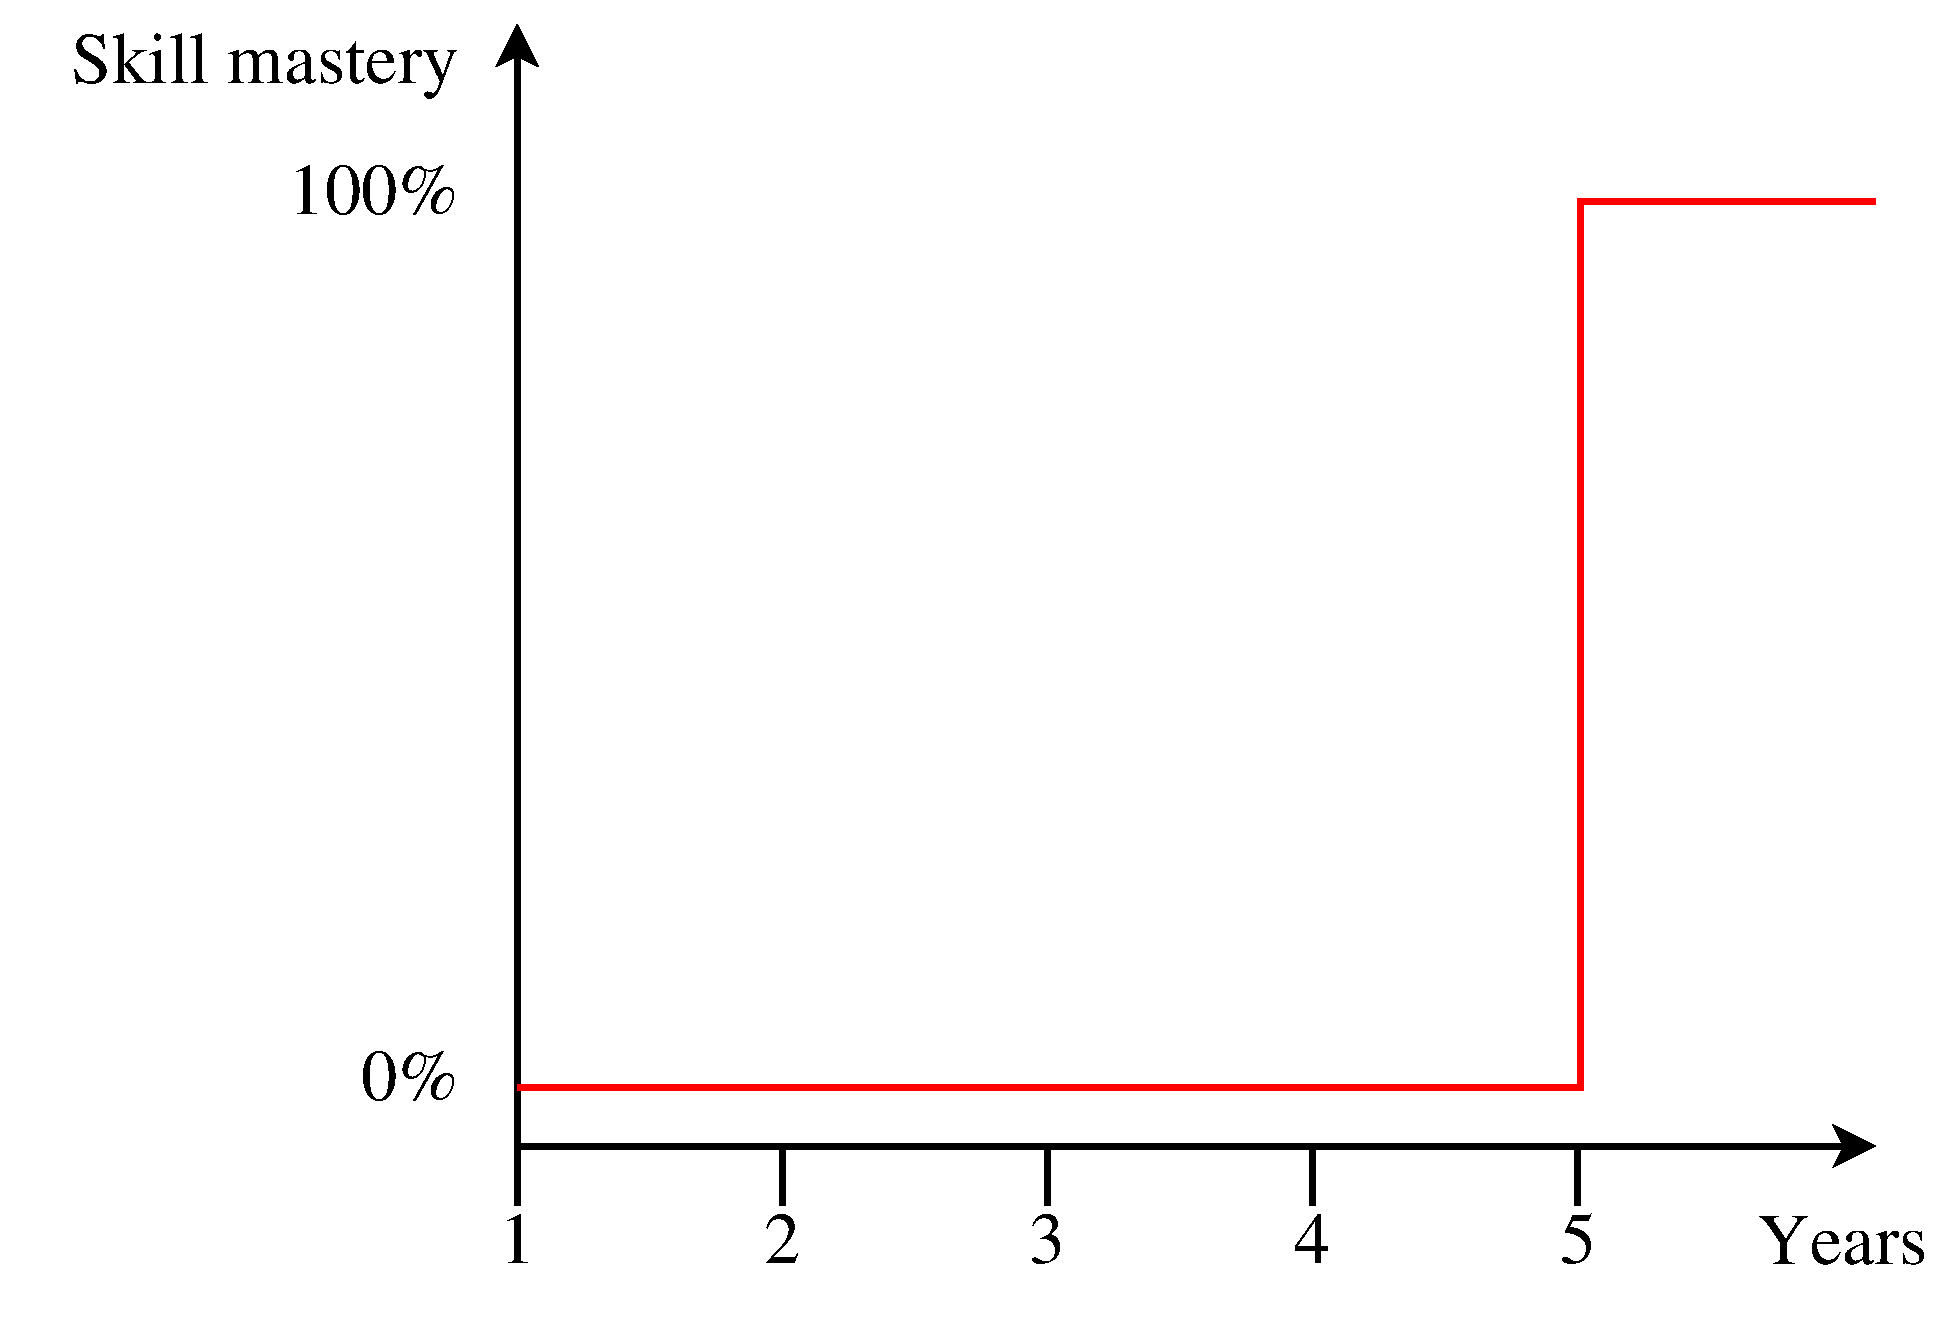
\includegraphics[width=\textwidth]{figures/learning-zigzag.eps}
	%          \rule{\textwidth}{0.5pt} % use line???
	\caption{Unrealistic}
	\label{}
	\end{subfigure}
	\begin{subfigure}{0.3\textwidth}
	\centering
	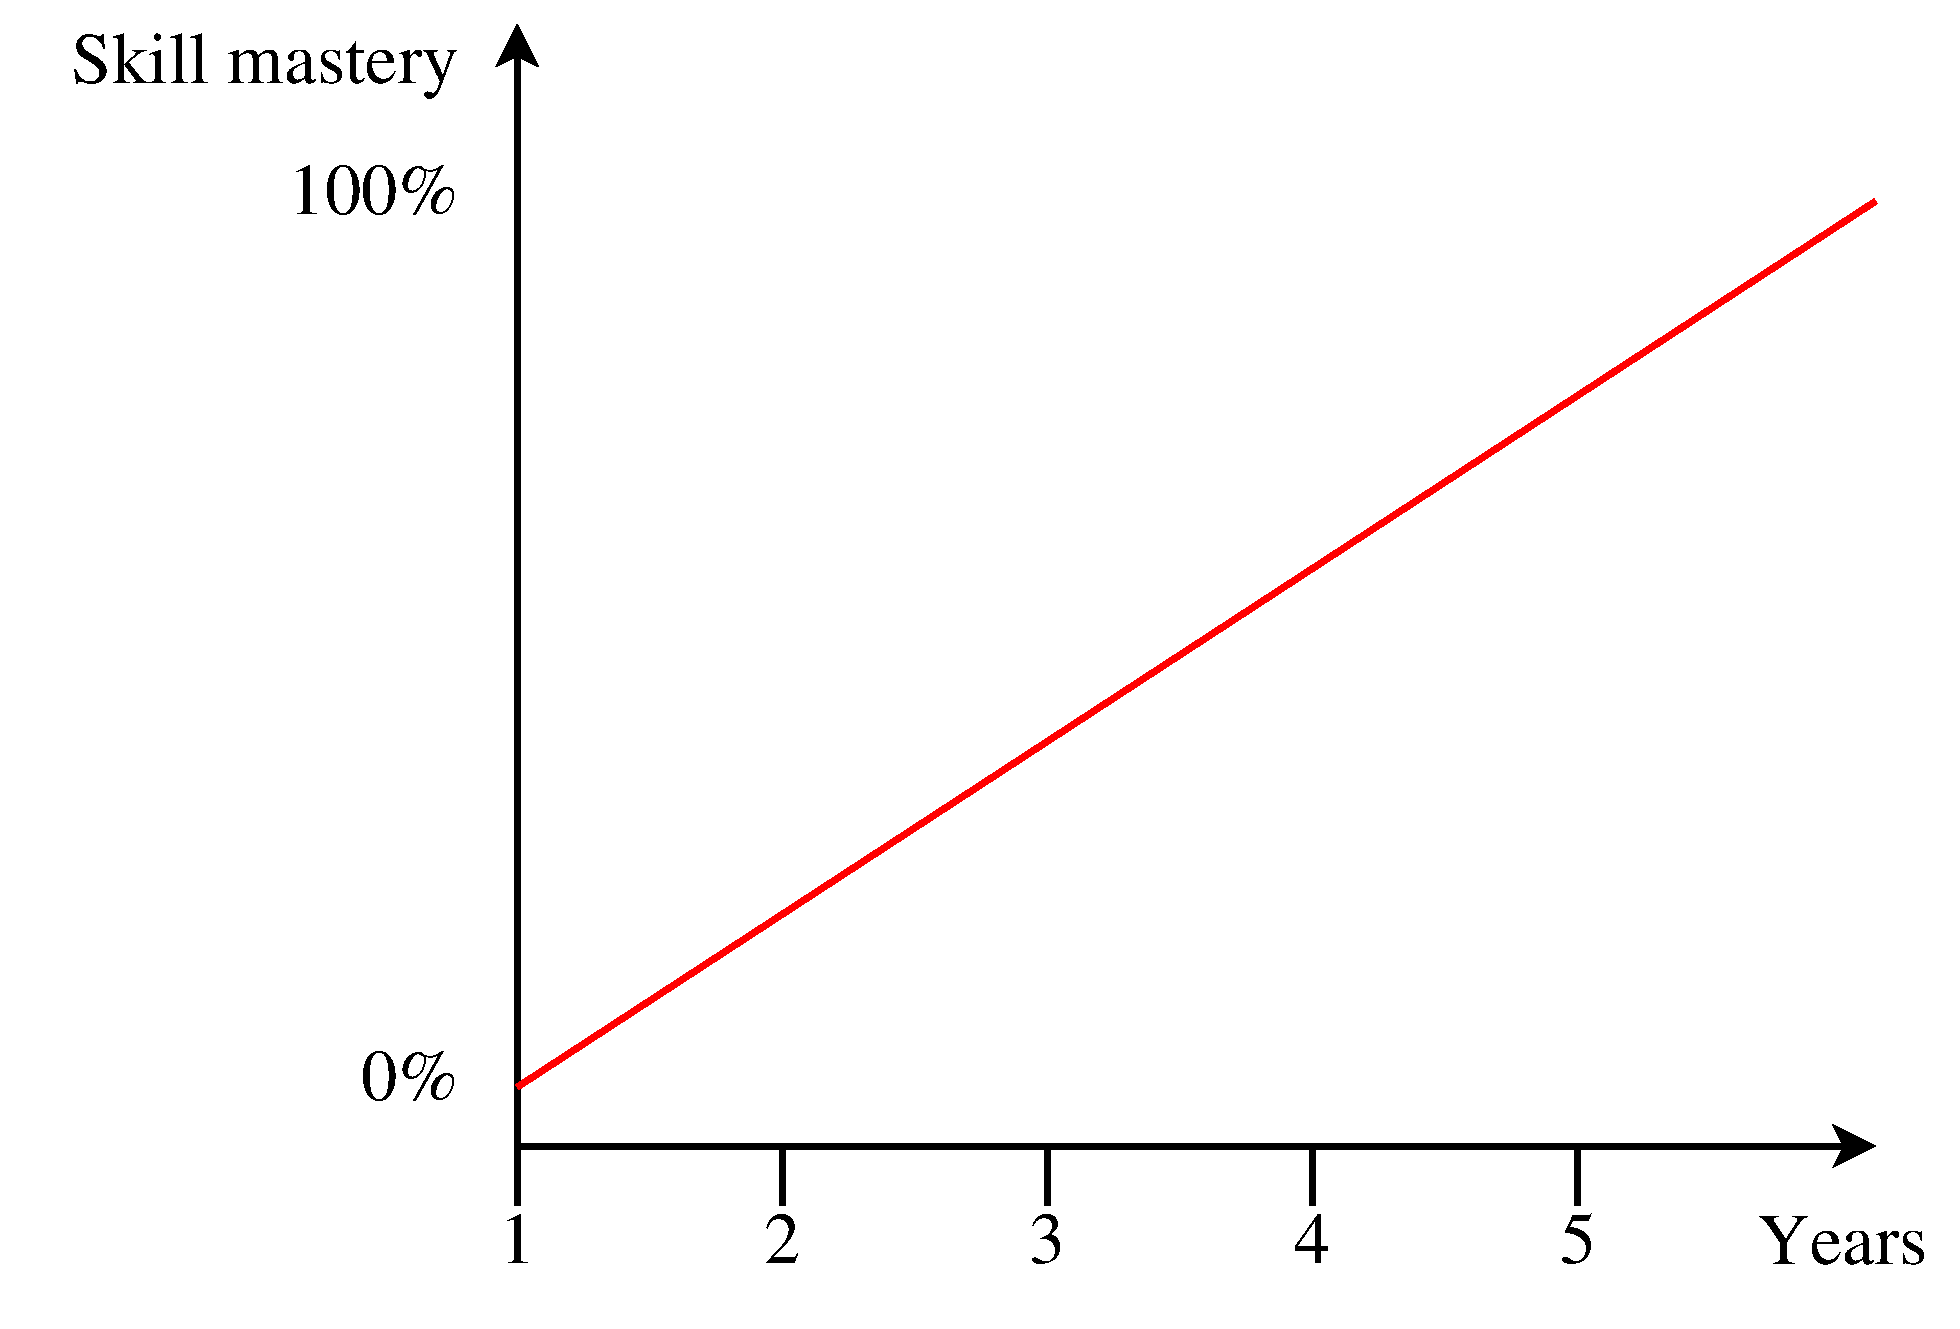
\includegraphics[width=\textwidth]{figures/learning-curve.eps}
	%          \rule{\textwidth}{0.5pt} % use line???
	\caption{Incremental}
	\label{}
	\end{subfigure}
	\rule{0.3\textwidth}{0.5pt} % use line???
	\caption{Ways to gain knowledge and understanding.}
	\label{}
	\end{wrapfigure}
\end{comment}



%\hl{Move following explanation to chapter intro?}
N.B. P2m is a LO for Masters students.
However, I do not think it is reasonable to assume that somebody can gain an extensive knowledge and understanding of a wide range of engineering materials and components (or most of anything) exclusively at Masters level, as shown in Figure~\ref{fig:learning01}.
I believe this is a cumulative process as shown in Figure~\ref{fig:learning02}, which is why, in my skills matrix, I have marked courses since Year 1 as having contributed to my attainment of this LO.


\begin{figure}[htbp]
	\centering
	\begin{subfigure}{.48\textwidth}
		\centering
		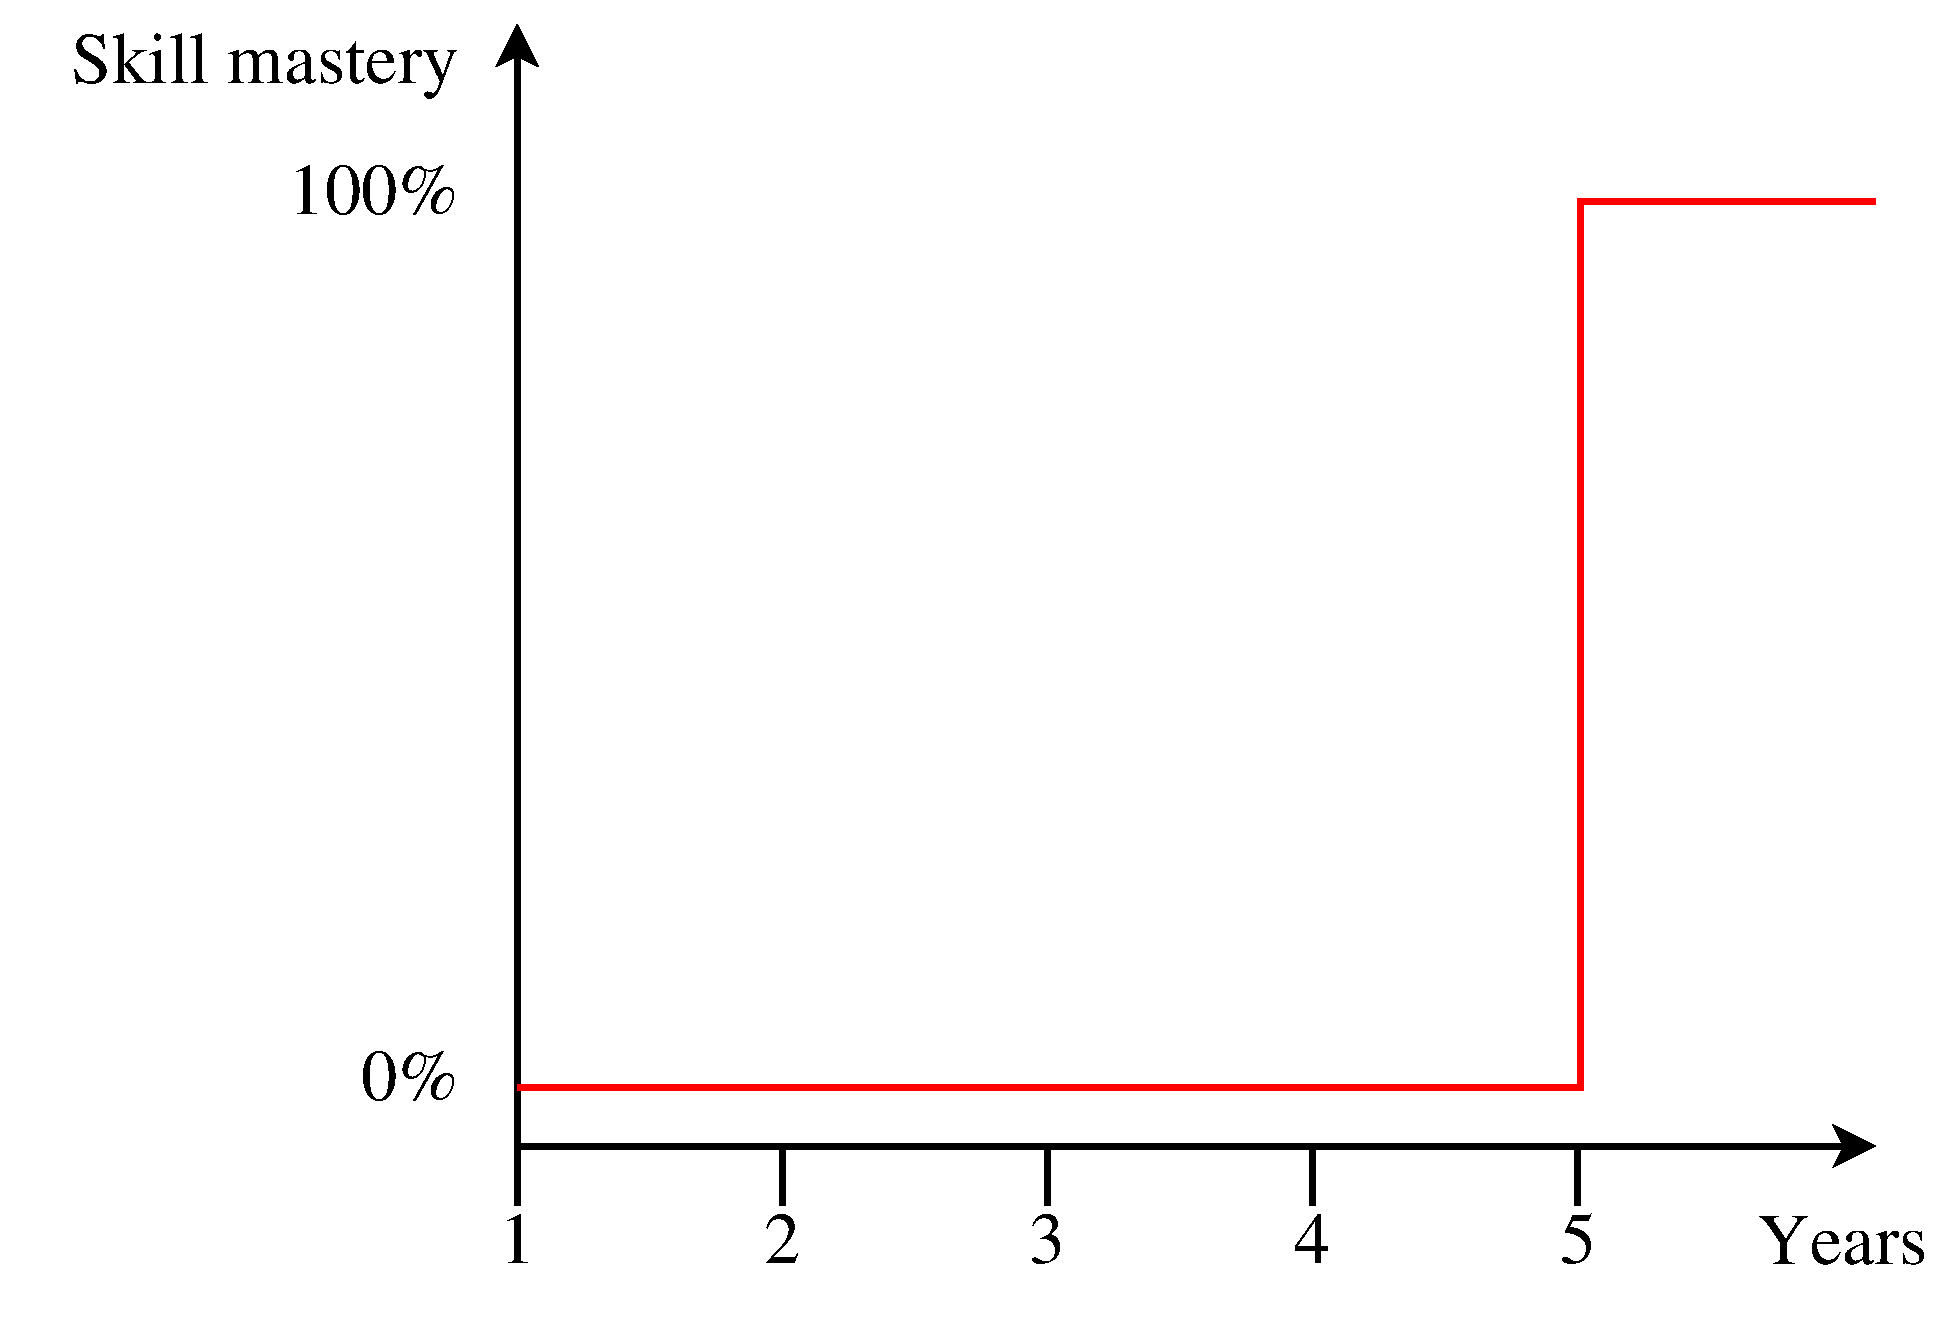
\includegraphics[width=0.75\textwidth]{figures/learning-zigzag.eps}
		%          \rule{\textwidth}{0.5pt} % use line???
		\caption{Unrealistic}
		\label{fig:learning01}
	\end{subfigure}
	\begin{subfigure}{.48\textwidth}
		\centering
		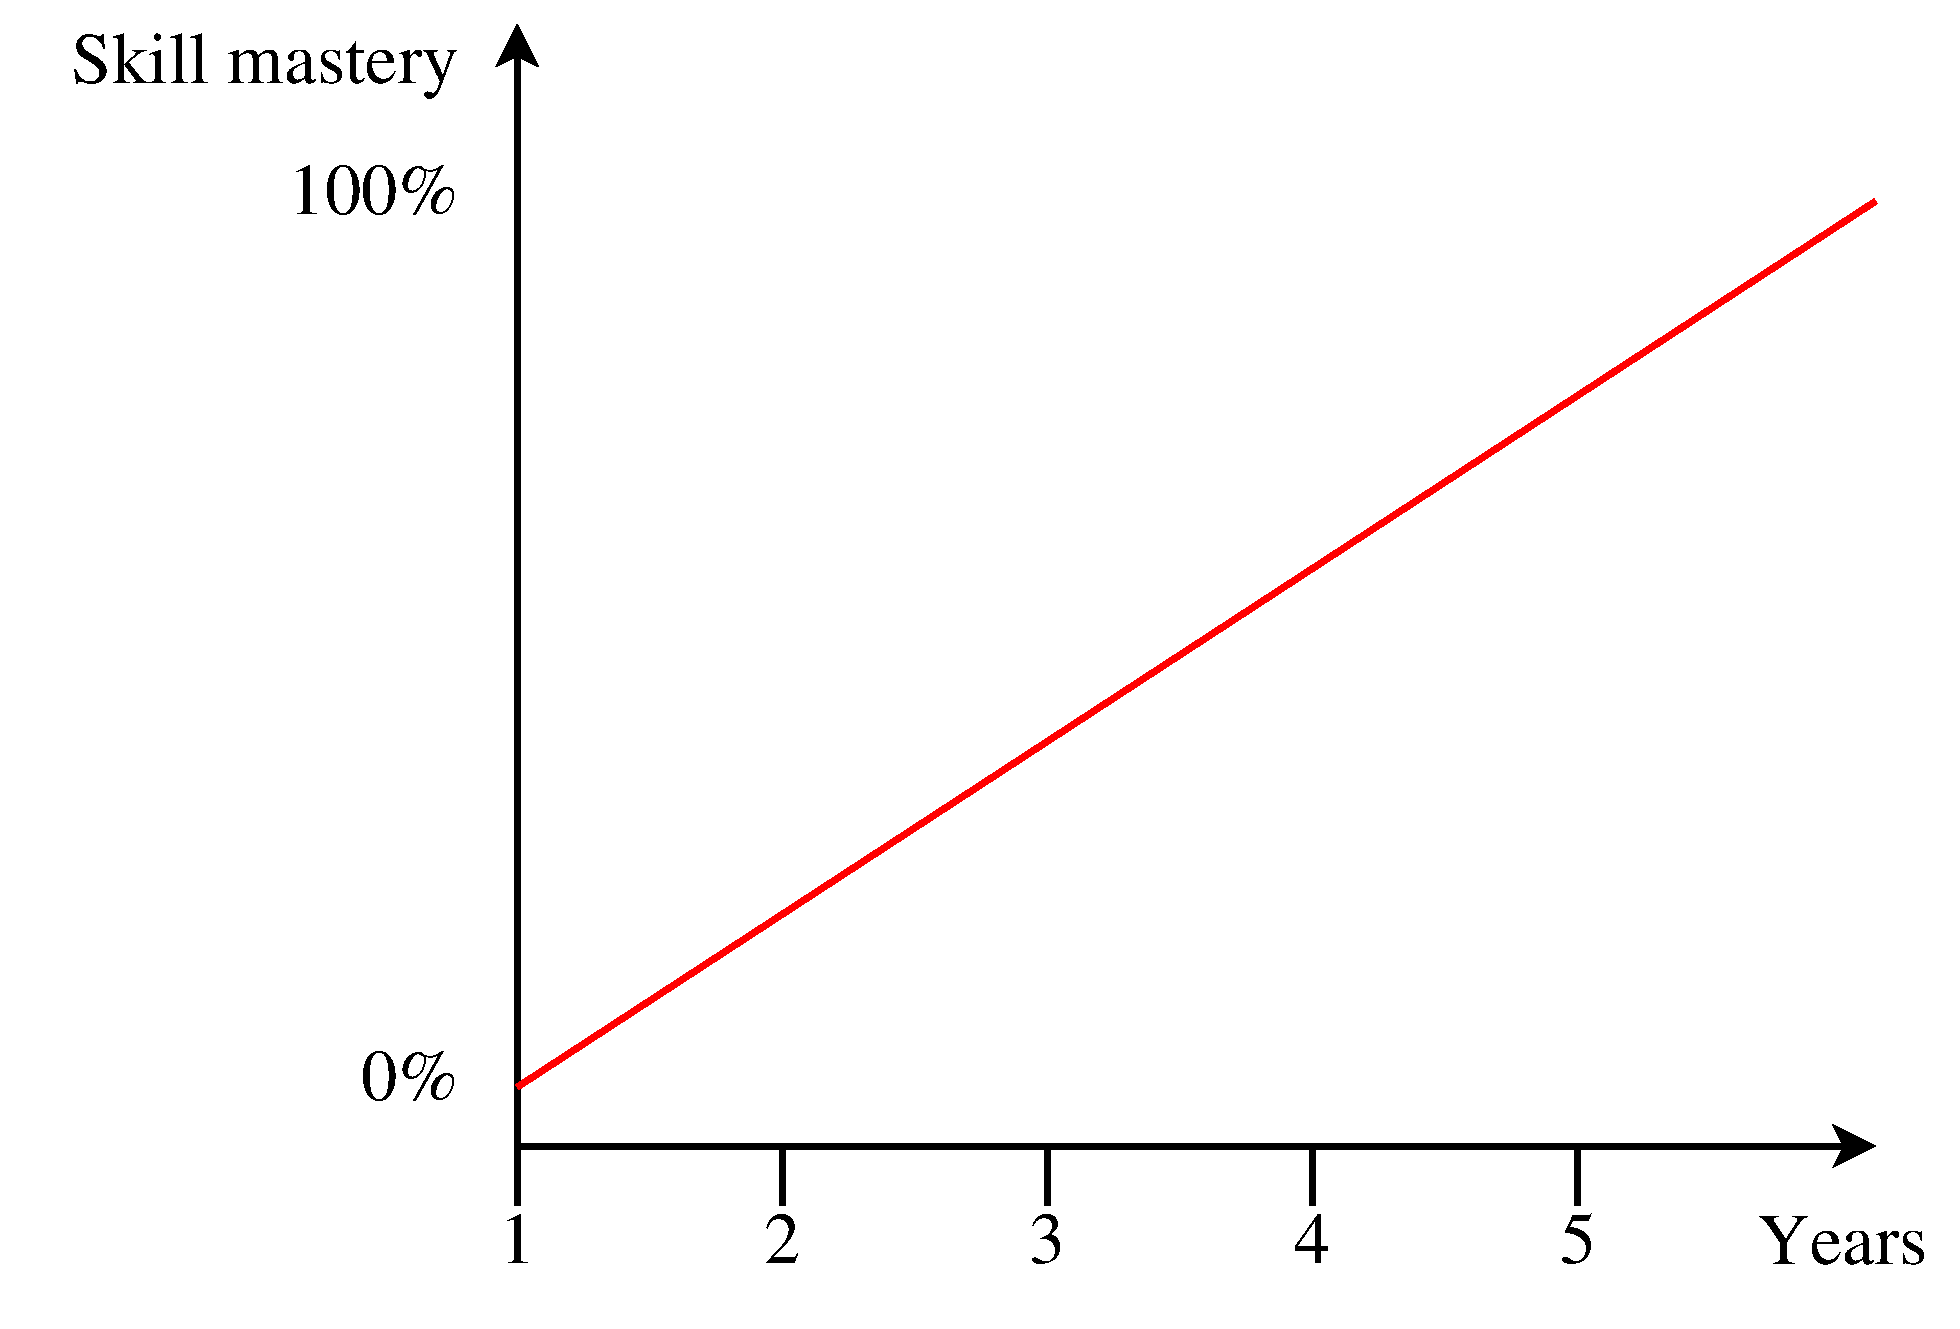
\includegraphics[width=0.75\textwidth]{figures/learning-curve.eps}
		%          \rule{\textwidth}{0.5pt} % use line???
		\caption{Incremental}
		\label{fig:learning02}
	\end{subfigure}
	\rule{\textwidth}{0.5pt} % use line???
	\caption{Ways to gain knowledge and understanding.}
	\label{fig:learning}
\end{figure}


%\hl{Write about increase in knowledge throughout the years. P2m for example couldn't all of a sudden have been achieved in Y5.}

%Building materials: insulation, steel, wood, Ziegel blocks, glass, PCMs etc.

%Building services products: ACs, HPs, PV, AHUs, Sunamp, windcatchers




\subsection*{P3(i, -)}

\begin{wraptable}{r}{0.2\textwidth}
    \begin{tabular}{|ll|}
        \hline
        \multicolumn{2}{|c|}{\cellcolor[HTML]{F8A102}\textbf{P3(i, -)} \master} \\ \hline
        \ConTechTwo & \Acoustics \\
        \HYD & \EPA \\
        \CAS & \TPS \\
        \LAB &  \\ \hline
    \end{tabular}
\end{wraptable}

%\begin{itemize}
%    \item \textbf{P3i}
    
    I have already had laboratory practice in physics, chemistry and biology in high school.
    In university, my knowledge and understanding of laboratory practice began to further develop in Year 2 when I conducted experiments in \textit{Construction Technology 2}, \textit{Acoustics and Architectural Design}, \textit{Hydraulics and Hydrology A} and \textit{Energy Principles and Applications} [\textbf{P3i}].
    The feedback for my hydraulics lab report of 93\% demonstrates my knowledge and understanding of laboratory practice.
    
%    \item \textbf{P3}
    
    In Years 3 and 4, I gained the ability to apply practical and laboratory skills that were more relevant to AE through my increased exposure to and application of laboratory practice in thermofluids and acoustics [\textbf{P3}].
    I re-visited the Services lab another two times for thermofluids-related experiments in \textit{Thermal Performance Studies} and \textit{Laboratory Project} and re-used my practical skills of recording, measuring and analysing sounds in \textit{Critical Architectural Studies} and \textit{Laboratory Project}.
%\end{itemize}

My final mark of 73\% in the \LABTitle \space demonstrates my full achievement of LOs P3i and P3.
%\hl{What actions and results can I show as evidence of my practical skills?}



\newpage
\subsection*{P4(i, -)}

\begin{wraptable}{r}{0.2\textwidth}
    \begin{tabular}{|l|}
        \hline
        \rowcolor[HTML]{F8A102} 
        \multicolumn{1}{|c|}{\cellcolor[HTML]{F8A102}\textbf{P4(i, -)} \littlemaster} \\ \hline
        \PRJ \\
        Sunamp \\ \hline
    \end{tabular}
\end{wraptable}

I have developed the ability to use and apply information from technical literature during my \PRJTitle \space and my Sunamp placement [\textbf{P4i}].
For the \PRJTitle, I sought, used and applied information from product specifications in order to size my building's water storage tank \citep{Decca}, calorifiers and buffer vessels \citep{RycroftLtd} etc.
At Sunamp, I used their technical manuals in order to produce the UniQ PISs (Appendix~\ref{App:PISs}).
%The technical literature I have been exposed to includes Sunamp's manuals for their UniQ product range and the product information sheets I drew up for them.
These sheets included information such as temperature input and output ranges, schematic diagrams, and the dimensions of the heat batteries.
%\hl{Include evidence, e.g. attach PISs}

%I also came across and used technical literature during my \textit{Design Project}.
%I used product specifications to size the college's water storage tank \citep{Decca}, calorifiers and buffer vessels \citep{RycroftLtd} etc.

Throughout my \textit{Design Project} and Sunamp experiences, I gained an understanding of the use of technical literature [\textbf{P4}].
%During the Design Project, I used technical literature to appropriately size some of the building services, both to accommodate the needs of the building's occupants and to fit inside of the plant room.
For example, at Sunamp, I was part of the decision-making process of the information that should be included in the UniQ PISs, which would be one of the first documents a customer would see once they have taken interest in Sunamp's products.
It was decided that information such as dimensions and weight were important to include for a couple reasons.
Firstly, to highlight the compact size of Sunamp's batteries (which is one of their unique selling points).
Secondly, to give the customers an indication of the transportation and placement requirements of a battery (e.g. depending on the type and size, a single UniQ battery will weigh between 55 kg and 211 kg 
%be it may need to be carried by two people and 
and will thus need to be placed on a load-bearing floor).
%\hl{Perhaps do not be afraid to write more sentences and give details such as specific weights and dimensions, and talk about stacking batteries and load bearing floors vs shelves etc.}


\subsection*{P5}

\begin{wraptable}{r}{0.2\textwidth}
	\begin{tabular}{|l|}
		\hline
		\rowcolor[HTML]{F8A102} 
		\multicolumn{1}{|c|}{\cellcolor[HTML]{F8A102}\textbf{P5} \littlemaster} \\ \hline
		\PC \\
		\DI \\ \hline
	\end{tabular}
\end{wraptable}

Considering that in the UK-SPEC defines knowledge as information that can be recalled, I do not have much knowledge of legal and contractual issues relevant to AE.
We have, however, covered contracts in \textit{Procurement and Contracts} and professional liability and insurance in \textit{Design Issues}.
It is perhaps due to a lack of coursework or examination and/ or a lack of spaced repetition of these topics throughout my degree programme that have I not gained a firm knowledge in relevant legal and contractual issues.





\subsection*{P6(i, -)}

\begin{wraptable}[5]{r}{0.2\textwidth}
	\begin{tabular}{|ll|}
		\hline
		\multicolumn{2}{|c|}{\cellcolor[HTML]{F8A102}\textbf{P6(i, -) \littlemaster}} \\ \hline
		\PRJ & \DST \\
		\ISE & H\&L \\
		Hoare Lea & Sweco \\ \hline
	\end{tabular}
\end{wraptable}

I have used appropriate codes of practice and industry standards during \textit{Design Project}, \textit{Inclusive and Safe Environments} and my placements at Hoare Lea and Sweco.
For the \textit{Design Project}, for example, I wanted to use water source heat pumps (WSHPs) to generate heat for the college I was designing since it was located right next to a body of water (see Figure \ref{fig:revit}).
I had to figure out how WSHPs could fit into the building's heating strategy.
To do this, I read about WHSPs in CIBSE CP2, the UK's Code of Practice for surface WSHPs.
I decided, because the college was a large non-domestic facility, to use a multi-valent heating system, where the WSHPs would provide the base heating load and some micro combined heat and power (CHP) units would satisfy the peak heating demands \citep[pp.~12,~38]{CP22016}.
%\hl{I have no feedback to demonstrate this specifically was good and my grade for DP wasn't good because of missing elements...}

I do not have a full understanding of appropriate codes of practice and industry standards as I have not had enough exposure to these.
My dissertation, however, has familiarised me with the UK BIM standards (particularly PAS 1192-2) quite well.
I believe my understanding will develop further once I start working in industry, as many of my building consultancy-type placements so far have required me to refer to such documents.






\subsection*{P7}

\begin{wraptable}{r}{0.2\textwidth}
    \begin{tabular}{|ll|}
        \hline
        \multicolumn{2}{|c|}{\cellcolor[HTML]{F8A102}\textbf{P7} \master} \\ \hline
        \EnvBeh & \CAS \\
        \FMP & \LAB \\
        \ICP & Sweco \\ \hline
    \end{tabular}
\end{wraptable}

I have gained an awareness of quality issues and their application to continuous improvement.
Regarding building services, perhaps the most pertinent example is the use of POEs.
POEs are useful ways to collect both objective and subjective data about the operation of a building, the purpose of which is to feed forward into the improvement of that and other buildings' performance.
For the design competition in \CASTitle, I took the initiative to create a POE in the form of a questionnaire which my group used to collect subjective data on the user and staff experiences of the Newington and Wester Hailes libraries in Edinburgh.
We used this data in our improved re-design of Newington Library to redress the problems that had been addressed.
For example, the old library fenestration design failed to exclude sunlight, which caused glare on computer monitors amongst other things.
Therefore, in my lighting and window design, I analysed the sun path and used frosted glazing on south-facing fa{\c{c}}ades to disperse rays of sunlight while maximising natural light.
% (although I am aware of this application).
%\hl{Get example of changes made and/ or include visual of POE questionnaire.}
The judges commended my natural lighting design (see Figure~\ref{fig_award}).
Overall, I believe I have fully achieved LO P7.

%CAS POE example
%technical examples: ICP, LAB thermo
%Sweco certification







\subsection*{P8}

\begin{wraptable}{r}{0.2\textwidth}
    \begin{tabular}{|ll|}
        \hline
        \multicolumn{2}{|c|}{\cellcolor[HTML]{F8A102}\textbf{P8} \littlemaster} \\ \hline
        \Stats & \TPS \\
        \PRJ & \\ \hline
    \end{tabular}
\end{wraptable}

I have a limited ability to work with technical uncertainty.
A lot of the work in the \PRJTitle, for example, was based on technical uncertainty, e.g. the design of drainage, water supply, heating and ventilation systems.
Having passed the course with a passing grade shows that I have some ability to work with technical uncertainty, but I have not yet mastered this skill.

%I think part of \hl{my failure?} of the Design Project was my inability to work with technical uncertainty.
%I have a tendency to be detail-oriented and thus get stuck in details etc., to not take risks and to be indecisive
%But I did (painstakingly) work through some uncertainties, thus achieving a passing grade (?).




\subsection*{P9m}

\begin{wraptable}{r}{0.2\textwidth}
    \begin{tabular}{|ll|}
        \hline
        \multicolumn{2}{|c|}{\cellcolor[HTML]{F8A102}\textbf{P9m} \littlemaster} \\ \hline
        \PC & \FMP \\
        \DST & \ICP \\ \hline
    \end{tabular}
\end{wraptable}

I have some understanding of current engineering practice and its limitations.
\PCTitle \space made me aware of some procurement routes (e.g. traditional, design and build, and Private Finance Initiative (PFI)) and contracts (notably the JCT (Joint Contracts Tribunal) standard forms of contract) that govern the execution of construction projects and the relationships between stakeholders etc.
% and the legal procedures \hl{when things get outta line}.
My dissertation, however, gave me the opportunity to delve into one aspect of current engineering practice in more detail, notably the collaboration induced by BIM in building services engineering.
%My dissertation assessed the effectiveness and implications of the UK industry’s BIM guidance in the context of building services engineering
My study revealed five discrepancies between industry guidance and practice in
building services engineers’ processes for collaboration in the UK.
Some of these discrepancies (between how the industry/ government says things should run and the way things are \emph{actually} running) are due to limitations.
For example, the industry recommends substituting \textit{generic} BIM objects with \textit{specific} BIM objects during equipment procurement, but this is technically not possible at the moment due to a lack of BIM software interoperability \citep{eklow_2018}.
My \DSTTitle \space mark of 83\% demonstrates my understanding of this collaborative aspect of current building services engineering practice.

%skill limitation:
%The third is the government’s request for early contractor involvement and the use of proprietary BIM objects from the outset of a project, which requires a practical knowledge and skill set.
%This conflicts with the purely theoretical knowledge and skill set of most consultants, if the consultants are the ones to be designing the building services at the start of a project.

\begin{wrapfigure}[7]{r}{0.3\textwidth}
	\centering
	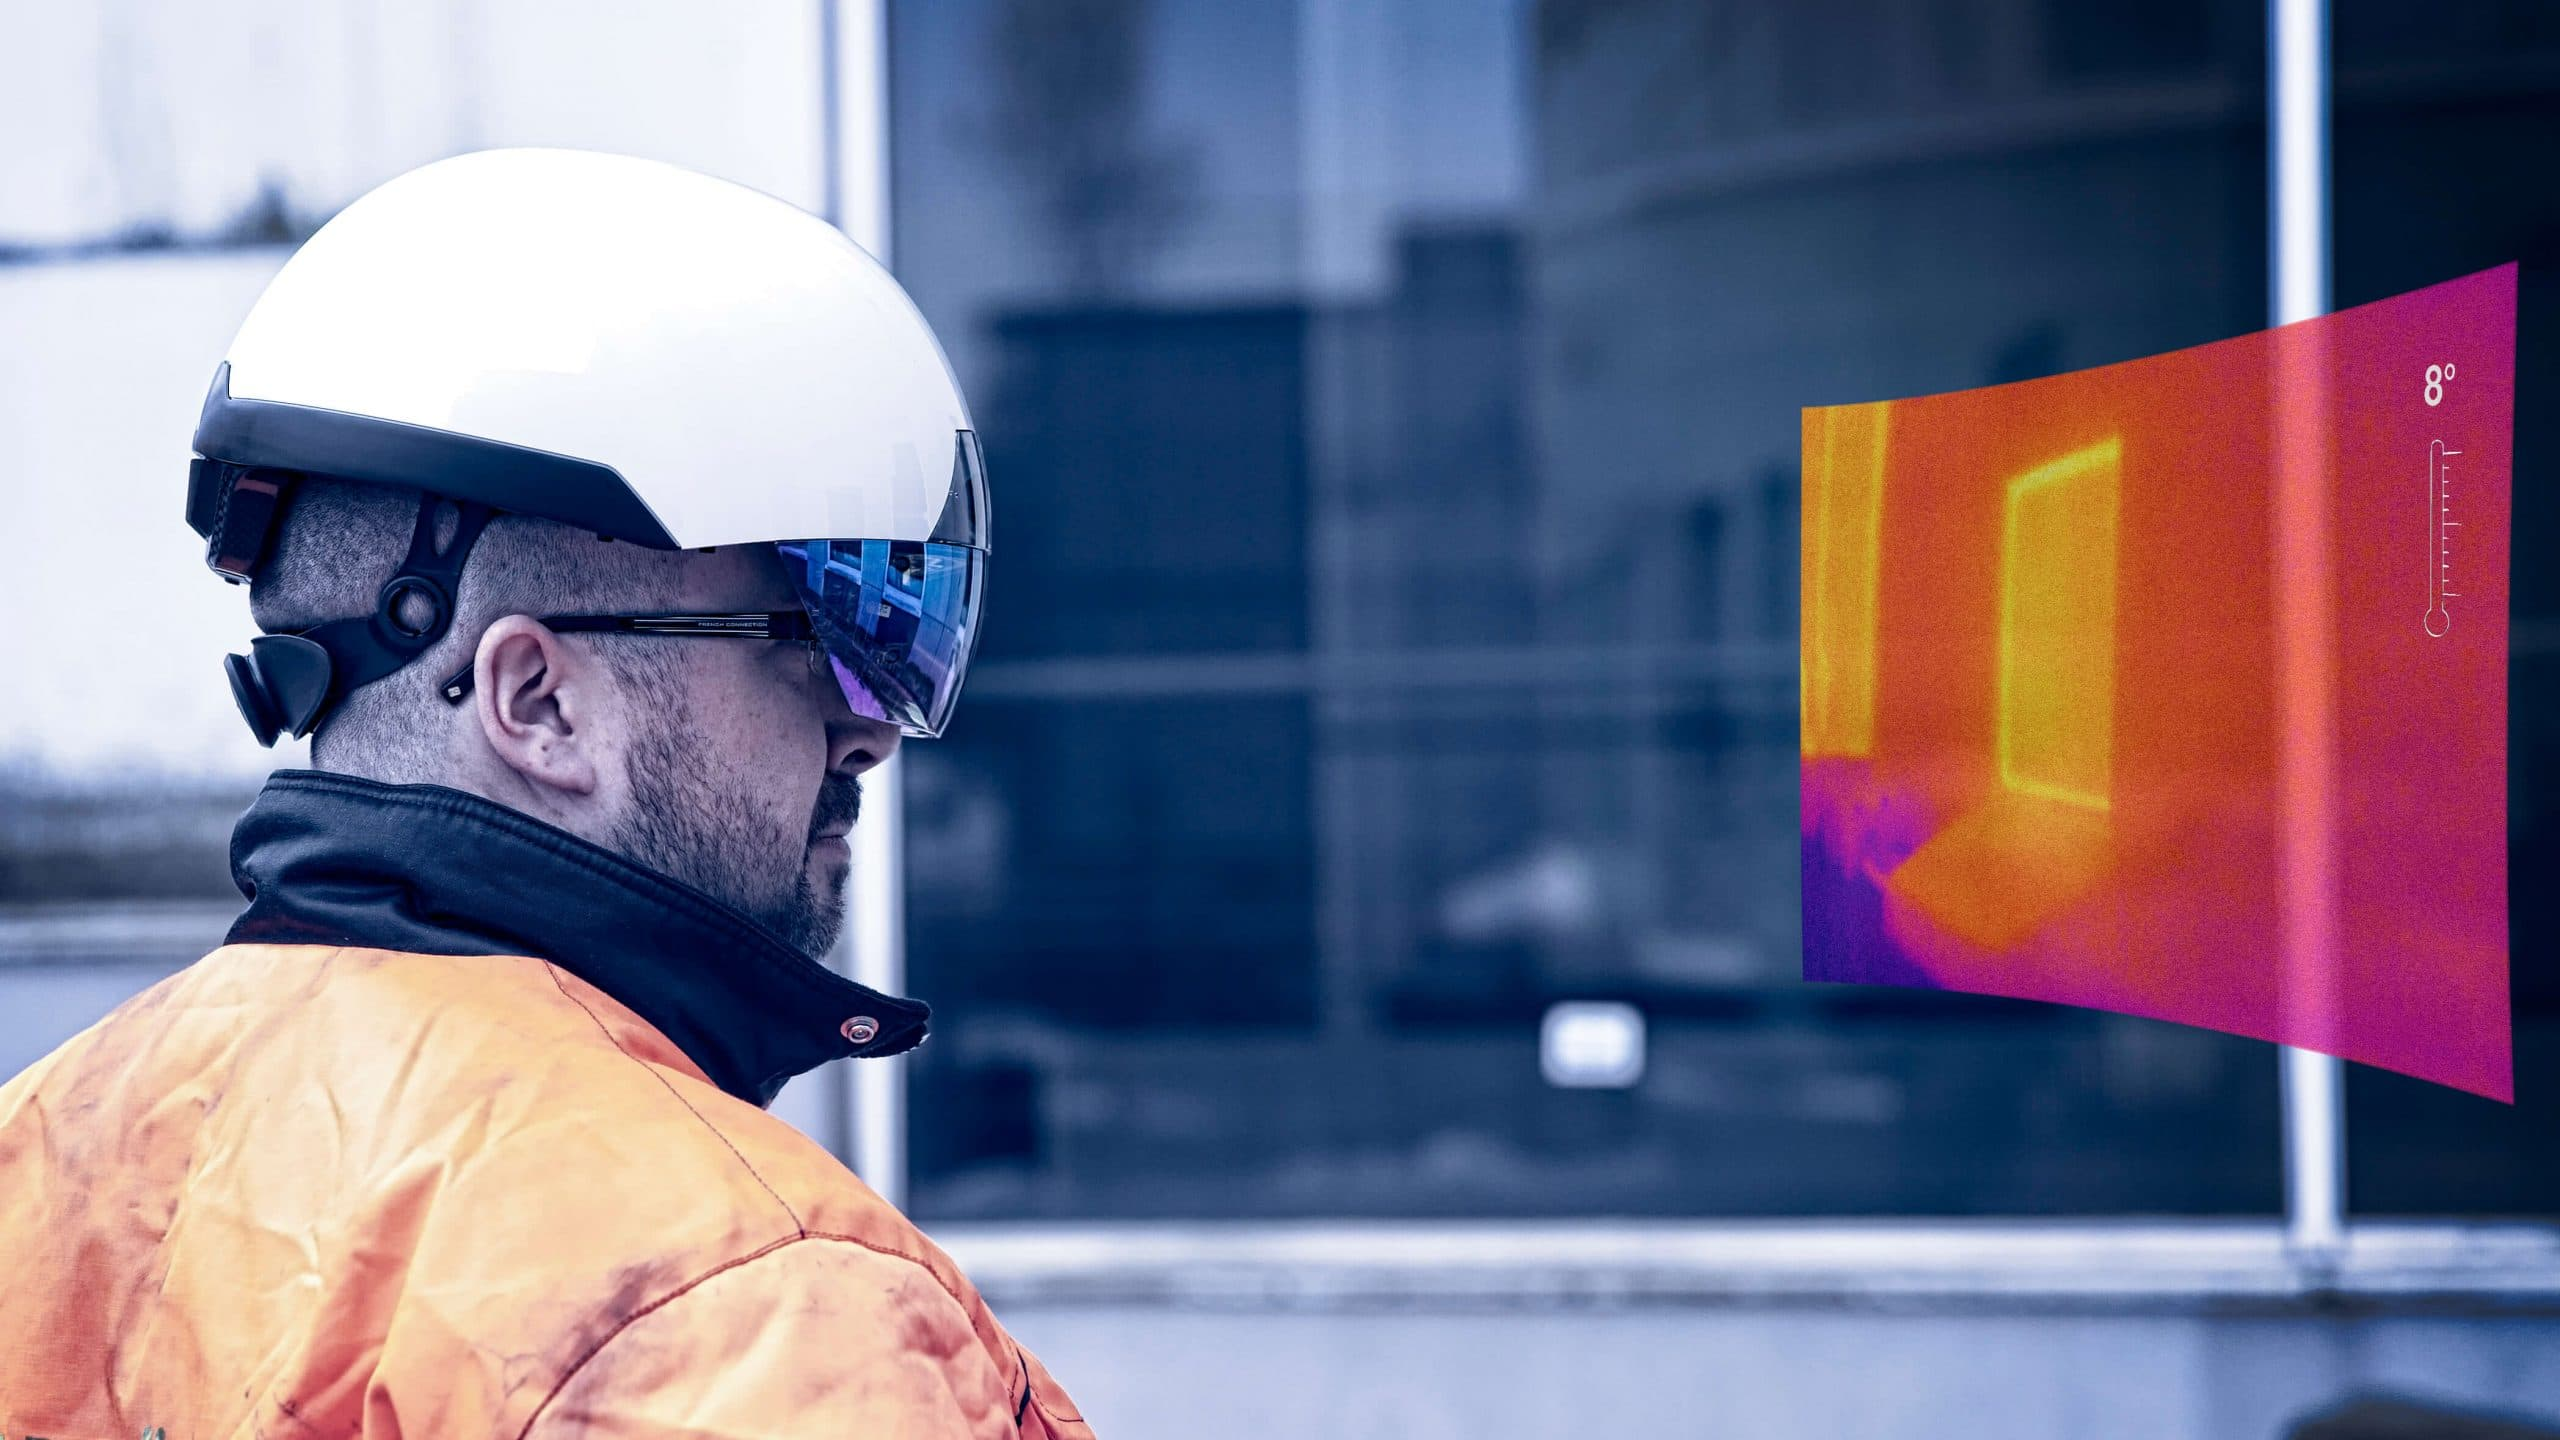
\includegraphics[width=0.3\textwidth]{figures/daqri.jpg}
	\rule{0.3\textwidth}{0.5pt} % use line???
	\caption[The Daqri Smart Helmet.]{The Daqri Smart Helmet \citep{DAQRI:stereoscape}.}
	\label{fig:daqri}
\end{wrapfigure}

I also have an appreciation of likely new developments, thanks to \ICPTitle.
This includes the use of virtual and augmented reality,
robotics,
modern methods of construction (MMC),
smart helmets (see Figure~\ref{fig:daqri}),
localisation and identification technologies (e.g. Global Navigation Satellite System (GNSS) and radio-frequency identification (RFID))
in construction.







\subsection*{P10m} \label{sec:P10m}

\begin{wraptable}{r}{0.2\textwidth}
    \begin{tabular}{|ll|}
        \hline
        \multicolumn{2}{|c|}{\cellcolor[HTML]{F8A102}\textbf{P10(i, b, m)} \littlemaster} \\ \hline
        \multicolumn{2}{|c|}{\PRJ} \\ \hline
    \end{tabular}
\end{wraptable}

I have on one occasion applied engineering techniques while taking account of commercial and industrial constraints.
During the 4\textsuperscript{th} year collaborative project (part of \PRJ), I used inspiration from the proposed Swansea Bay Tidal Lagoon in South West Wales to suggest a way to generate tidal power on our building site
(see a video demonstrating the tidal lagoon concept here: \url{http://www.tidallagoonpower.com/projects/swansea-bay/3d-model/}).
As I was researching the tidal technology, I discovered that the hydro turbines needed to be bi-directional (i.e. work in reverse) in order to take advantage of both the ebb and flood tides \citep{TurbineTech}, but that such turbines were not readily available on the market. 
%\hl{(source cannot currently be found).}
Therefore my group allocated a substantial amount of the budget to the manufacture of custom turbines, such as by Andritz Hydro \citep{TurbineTech}.

%I also attempted to study the viability of tidal power generation at the building site by calculating the potential annual yield of a tidal lagoon set-up.
%Because this is a fairly new technology, I struggled to find calculation methods.
%I eventually had to make assumptions and I used a yield equation for hydroelectricity (? \hl{find calcs and scan in!}).

This is the only example I can think of that demonstrates my achievement (if partial) of P10m.
Since it is a Masters level LO, I will hopefully get opportunities to further develop this ability in Semester 2 of Year 5, or when I start to work in industry.





\subsection*{P11(i, b, m)}

% Similar to G4

\begin{wraptable}{r}{0.2\textwidth}
    \begin{tabular}{|ll|}
        \hline
        \multicolumn{2}{|c|}{\cellcolor[HTML]{F8A102}\textbf{P11(i, b, m)} \nomaster} \\ \hline
        \CAS & \TPS \\
        \PRJ & \LAB \\
        Arup & Hoare Lea \\
        \multicolumn{2}{|l|}{Hultin \& Lundquist} \\ \hline
    \end{tabular}
\end{wraptable}

Every year, my ability to work as a team member in the role of an architectural engineer has increased, as has my awareness of the team roles of a building design team (a type of engineering team) [\textbf{P11i}].
This is thanks to my involvement in almost annual cross-disciplinary design projects, notably the 2\textsuperscript{nd} year and 4\textsuperscript{th} year collaborative projects, and the design project in \CASTitle, and my attendance at design team meetings at some of my placements.
The roles of a building design team include:
\begin{itemize}
    \item Urban planners, who look at the overall socio-economic aspects of urban development and consider the benefits and viability of constructing a building in a certain area
    \item Quantity surveyors, who calculate the costs of a building project
    \item Structural and civil engineers, who design the sub- and superstructure of a building, ensuring the whole structure is supportive and resilient
    \item Architectural engineers (a.k.a. building services engineers), who make the building usable and comfortable, and whose work greatly influences the operational energy consumption and costs
    \item Interior designers, who style the building interior
    \item Construction project managers, who supervise and coordinate the efforts of the construction workers on site
\end{itemize}


\begin{figure}[htbp]
	\centering
	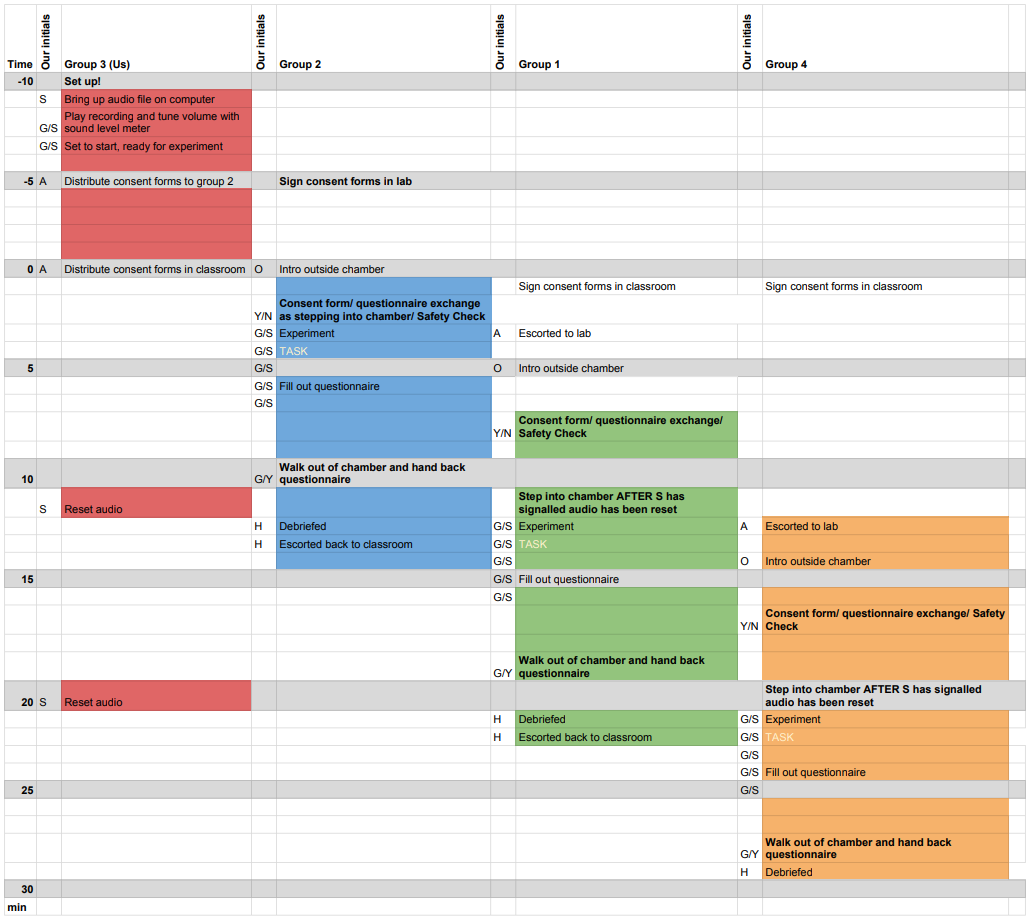
\includegraphics[width=0.5\textwidth]{figures/lab-gantt.PNG}
	\rule{\textwidth}{0.5pt} % use line???
	\caption[Acoustics experiment programme.]{The programme I created to coordinate my group in an acoustics laboratory experiment (\LAB).}
	\label{fig:lab-gantt}
\end{figure}



My ability to exercise personal responsibility as a member of an engineering team can be demonstrated by my contribution to the passive design (e.g. natural lighting) of a library building, which helped our group win the 1\textsuperscript{st} prize in sustainability in \CASTitle \space (see Figure~\ref{fig_award}).

Apart from AE, the only other team role I may have a partial understanding of is that of the project manager.
This is due to my frequent experiences of leading and coordinating a team in group projects,
%\hl{(example?)}, 
as well as my self-initiated attempts to use a Gantt-\textit{esque} chart to plan the timeline of a group-conducted acoustics experiment in \LABTitle \space (see Figure~\ref{fig:lab-gantt})
and
my dissertation work (see Figure~\ref{DST_schedule}) [\textbf{P11b and P11m}].

Unfortunately, I have not come as far as to understand the other aforementioned roles of a building design team.
This is because I have not had experience using my knowledge (albeit limited) of those roles.
Regarding quantity surveying, I have had at least two opportunities to try out that role (in the \CASTitle \space design project and the \PRJTitle), but I did not use these opportunities.
Another opportunity I missed that may have improved my understanding of some of these roles is \textit{Constructionarium}, a week-long, on-site and hands-on construction project where a team of students replicate an existing structure (e.g. a tower or bridge) in miniature scale.